\documentclass[11pt,a4paper]{article}
\usepackage[margin=2.3cm]{geometry}
\usepackage{amsmath,amssymb,bm}
\usepackage{graphicx}
\usepackage{booktabs}
\usepackage{siunitx}
\usepackage{listings}
\usepackage{xcolor}
\usepackage{tikz}
\usetikzlibrary{positioning,arrows.meta,calc}
\usepackage{caption}
\captionsetup{font=small,labelfont=bf}

\newcommand{\Rfrac}{12}
\newcommand{\hlay}{10}
\newcommand{\dxcell}{20}
\newcommand{\dleak}{5}
\newcommand{\permmD}{100}
\newcommand{\muCp}{0.5}
\newcommand{\rhor}{1020}
\newcommand{\Qbase}{8}
\newcommand{\gammabase}{0.004}
\newcommand{\gammabaseh}{0.4}
\newcommand{\WoverL}{100}
\newcommand{\Emod}{10}
\newcommand{\nupois}{0.25}
\newcommand{\pnet}{2.0}
\newcommand{\wmax}{0.57}
\newcommand{\sigmagrad}{0.17}
\newcommand{\Atop}{109.8}
\newcommand{\Amid}{232.9}
\newcommand{\Abot}{109.8}
\newcommand{\Atot}{452.4}
\newcommand{\Ltop}{74.9}
\newcommand{\Lmid}{158.8}
\newcommand{\Lbot}{74.9}
\newcommand{\Ltot}{308.6}
\newcommand{\Mk}{29.1}
\newcommand{\ro}{3.96}
\newcommand{\Wcond}{30860}
\newcommand{\phiwref}{0.0278}
\newcommand{\phiFref}{0.0181}
\newcommand{\qftop}{1.28}
\newcommand{\qfmid}{3.01}
\newcommand{\qfbot}{1.28}
\newcommand{\qfnodetop}{1.28}
\newcommand{\qfnodemid}{3.01}
\newcommand{\qfnodebot}{1.28}
\newcommand{\qmtop}{0.81}
\newcommand{\qmmid}{0.81}
\newcommand{\qmbot}{0.81}
\newcommand{\Ttop}{46.2}
\newcommand{\Tmid}{108.4}
\newcommand{\Tbot}{46.2}
\newcommand{\TLtop}{0.617}
\newcommand{\TLmid}{0.683}
\newcommand{\TLbot}{0.617}
\newcommand{\dptop}{0.0278}
\newcommand{\dpmid}{0.0278}
\newcommand{\dpbot}{0.0278}
\newcommand{\phiwA}{0.0278}
\newcommand{\qAtop}{2.09}
\newcommand{\qAmid}{3.82}
\newcommand{\qAbot}{2.09}
\newcommand{\sTopv}{0.040}
\newcommand{\sBotv}{-0.040}
\newcommand{\phiwC}{0.0278}
\newcommand{\qCftop}{3.13}
\newcommand{\qCfmid}{3.01}
\newcommand{\qCfbot}{-0.56}
\newcommand{\qCmtop}{1.97}
\newcommand{\qCmmid}{0.81}
\newcommand{\qCmbot}{-0.36}
\newcommand{\qCtop}{5.10}
\newcommand{\qCmid}{3.82}
\newcommand{\qCbot}{-0.92}
\newcommand{\Qcrit}{11.5}
\newcommand{\Ttot}{288.1}
\newcommand{\sseedtop}{1.000}
\newcommand{\Qcritseed}{288}
\newcommand{\qseedtop}{77.4}
\newcommand{\qseedmid}{3.8}
\newcommand{\qseedbot}{-73.2}
\newcommand{\pwqbzero}{0.0407}
\newcommand{\deltab}{0.03}
\newcommand{\remLtop}{5.10}
\newcommand{\remLbot}{-0.92}
\newcommand{\remTwotop}{3.65}
\newcommand{\remTwomid}{4.55}
\newcommand{\remTwobot}{-0.20}
\newcommand{\remTwoTbot}{0.0}
\newcommand{\remThrtop}{3.26}
\newcommand{\remThrmid}{3.82}
\newcommand{\remThrbot}{0.93}
\newcommand{\remThrfbot}{1.28}
\newcommand{\remThrmbot}{-0.36}
\newcommand{\dynLbot}{-0.64}
\newcommand{\dynLtop}{4.91}
\newcommand{\dynTbot}{2.16}
\newcommand{\Cstore}{8}
\newcommand{\Aqsup}{1000}
\newcommand{\codeQcrit}{11.7}
\newcommand{\dpdrop}{0.0097}
\newcommand{\dynFbot}{1.10}
\newcommand{\dynTwobot}{-0.09}
\newcommand{\qCNtop}{6.26}
\newcommand{\qCNmid}{3.80}
\newcommand{\qCNbot}{-2.06}
\newcommand{\alphaCN}{1.000}
\newcommand{\phiwCN}{0.0202}
\newcommand{\shareCN}{1.54}
\newcommand{\QcritCN}{15.9}
\newcommand{\qfCNbot}{-1.48}
\newcommand{\qmCNbot}{-0.58}
\newcommand{\qCDtop}{4.34}
\newcommand{\qCDmid}{3.40}
\newcommand{\qCDbot}{0.26}
\newcommand{\alphaCD}{0.293}
\newcommand{\phiwCD}{0.0450}
\newcommand{\shareCD}{0.45}
\newcommand{\QcritCD}{6.7}
\newcommand{\qfCDbot}{0.11}
\newcommand{\qmCDbot}{0.15}
\newcommand{\qCFtop}{5.27}
\newcommand{\qCFmid}{3.68}
\newcommand{\qCFbot}{-0.95}
\newcommand{\alphaCF}{0.651}
\newcommand{\phiwCF}{0.0278}
\newcommand{\shareCF}{1.00}
\newcommand{\QcritCF}{11.7}
\newcommand{\qfCFbot}{-0.60}
\newcommand{\qmCFbot}{-0.36}
\newcommand{\qCGtop}{4.34}
\newcommand{\qCGmid}{3.40}
\newcommand{\qCGbot}{0.26}
\newcommand{\alphaCG}{0.293}
\newcommand{\phiwCG}{0.0450}
\newcommand{\shareCG}{0.45}
\newcommand{\QcritCG}{7.7}
\newcommand{\qfCGbot}{0.11}
\newcommand{\qmCGbot}{0.15}
\newcommand{\QcritNonormAn}{15.8}
\newcommand{\QcritFloorAn}{6.7}
\newcommand{\pfloor}{0.10}
\newcommand{\gsum}{200.8}
\newcommand{\Msum}{87.4}
\newcommand{\dynCDbot}{0.38}
\newcommand{\dynCDtop}{4.26}
\newcommand{\dynCNbot}{-1.59}
\newcommand{\dynCNtop}{5.94}
\newcommand{\dynCGbot}{0.38}
\newcommand{\dynCGtop}{4.26}

\newcommand{\Wrhow}{1004}
\newcommand{\Wmu}{0.398}
\newcommand{\WBw}{1.0219}
\newcommand{\WQ}{102.2}
\newcommand{\WQs}{100}
\newcommand{\WR}{3}
\newcommand{\Wpnet}{20}
\newcommand{\Wwmax}{0.96}
\newcommand{\Wdleak}{0.5}
\newcommand{\Wrw}{0.108}
\newcommand{\Wro}{0.396}
\newcommand{\WD}{1.299}
\newcommand{\WM}{207}
\newcommand{\WLtot}{2422}
\newcommand{\WLmid}{1007}
\newcommand{\WLnb}{707}
\newcommand{\Wlpa}{85.6}
\newcommand{\Wphiw}{0.0315}
\newcommand{\Whyd}{0.197}
\newcommand{\Wratio}{6}
\newcommand{\WTtot}{3241}
\newcommand{\WTleg}{2206}
\newcommand{\Wgcl}{0.0080}
\newcommand{\Wgcc}{0.0150}
\newcommand{\Wgclpct}{8.1}
\newcommand{\Wgamma}{0.030}
\newcommand{\Wdsig}{388}
\newcommand{\Wsig}{330}
\newcommand{\Wpres}{192.5}
\newcommand{\Wbeta}{0.0046}
\newcommand{\WAq}{110}
\newcommand{\WTv}{430}
\newcommand{\WC}{2}
\newcommand{\WKkc}{100}
\newcommand{\Wconc}{10}
\newcommand{\Wkc}{10}
\newcommand{\Wphic}{0.3}
\newcommand{\WRefNbotfirst}{10.53}
\newcommand{\WRefNbotlast}{10.54}
\newcommand{\WRefNtopfirst}{10.53}
\newcommand{\WRefNtoplast}{10.54}
\newcommand{\WRefNminfirst}{10.53}
\newcommand{\WRefNminlast}{10.54}
\newcommand{\WRefNphiwlast}{0.224}
\newcommand{\WRefNQcfirst}{389}
\newcommand{\WRefNQclast}{389}
\newcommand{\WRefDbotfirst}{10.53}
\newcommand{\WRefDbotlast}{3.85}
\newcommand{\WRefDtopfirst}{10.53}
\newcommand{\WRefDtoplast}{3.85}
\newcommand{\WRefDminfirst}{10.53}
\newcommand{\WRefDminlast}{3.85}
\newcommand{\WRefDphiwlast}{0.255}
\newcommand{\WRefDQcfirst}{389}
\newcommand{\WRefDQclast}{223}
\newcommand{\WLegNbotfirst}{-2.51}
\newcommand{\WLegNbotlast}{-2.51}
\newcommand{\WLegNtopfirst}{23.57}
\newcommand{\WLegNtoplast}{23.31}
\newcommand{\WLegNminfirst}{-2.51}
\newcommand{\WLegNminlast}{-2.51}
\newcommand{\WLegNphiwlast}{0.223}
\newcommand{\WLegNQcfirst}{389}
\newcommand{\WLegNQclast}{398}
\newcommand{\WLegDbotfirst}{-2.51}
\newcommand{\WLegDbotlast}{-0.49}
\newcommand{\WLegDtopfirst}{23.57}
\newcommand{\WLegDtoplast}{4.91}
\newcommand{\WLegDminfirst}{-2.51}
\newcommand{\WLegDminlast}{-0.49}
\newcommand{\WLegDphiwlast}{0.241}
\newcommand{\WLegDQcfirst}{389}
\newcommand{\WLegDQclast}{303}
\newcommand{\WConNbotfirst}{0.69}
\newcommand{\WConNbotlast}{-0.54}
\newcommand{\WConNtopfirst}{28.57}
\newcommand{\WConNtoplast}{26.72}
\newcommand{\WConNminfirst}{0.69}
\newcommand{\WConNminlast}{-0.54}
\newcommand{\WConNphiwlast}{0.239}
\newcommand{\WConNQcfirst}{202}
\newcommand{\WConNQclast}{247}
\newcommand{\WConDbotfirst}{0.69}
\newcommand{\WConDbotlast}{1.66}
\newcommand{\WConDtopfirst}{28.57}
\newcommand{\WConDtoplast}{5.67}
\newcommand{\WConDminfirst}{0.69}
\newcommand{\WConDminlast}{1.66}
\newcommand{\WConDphiwlast}{0.274}
\newcommand{\WConDQcfirst}{202}
\newcommand{\WConDQclast}{164}
\newcommand{\WOptNbotfirst}{-5.51}
\newcommand{\WOptNbotlast}{-5.43}
\newcommand{\WOptNtopfirst}{26.58}
\newcommand{\WOptNtoplast}{26.50}
\newcommand{\WOptNminfirst}{-5.51}
\newcommand{\WOptNminlast}{-5.43}
\newcommand{\WOptNphiwlast}{0.224}
\newcommand{\WOptNQcfirst}{124}
\newcommand{\WOptNQclast}{124}
\newcommand{\WOptDbotfirst}{-5.51}
\newcommand{\WOptDbotlast}{-1.87}
\newcommand{\WOptDtopfirst}{26.58}
\newcommand{\WOptDtoplast}{5.82}
\newcommand{\WOptDminfirst}{-5.51}
\newcommand{\WOptDminlast}{-1.87}
\newcommand{\WOptDphiwlast}{0.261}
\newcommand{\WOptDQcfirst}{124}
\newcommand{\WOptDQclast}{30}
\newcommand{\WgssLeg}{0.024}
\newcommand{\WgssdLeg}{0.031}
\newcommand{\WgsspctLeg}{24}
\newcommand{\WskewLegtop}{14.9}
\newcommand{\WskewLegbot}{6.2}
\newcommand{\WgssCon}{0.029}
\newcommand{\WgssdCon}{0.035}
\newcommand{\WgsspctCon}{29}
\newcommand{\WskewContop}{17.6}
\newcommand{\WskewConbot}{8.5}
\newcommand{\WgssOpt}{0.020}
\newcommand{\WgssdOpt}{0.026}
\newcommand{\WgsspctOpt}{20}
\newcommand{\WskewOpttop}{15.9}
\newcommand{\WskewOptbot}{5.2}
\newcommand{\WLegDqfTop}{57.3}
\newcommand{\WLegDqmodTop}{-0.9}
\newcommand{\WLegDTTop}{966}
\newcommand{\WLegDLrelTop}{1.00}
\newcommand{\WLegDLrelBot}{0.52}
\newcommand{\WLegDmBot}{1.00}
\newcommand{\WLegDphiTop}{0.242}
\newcommand{\WLegDphiw}{0.241}
\newcommand{\WLzero}{707}
\newcommand{\WLegNqfTop}{33.7}
\newcommand{\WLegNqmodTop}{-8.6}
\newcommand{\WLegNqfLow}{8.3}
\newcommand{\WLegNqmodLow}{48.1}
\newcommand{\WLegNphiTop}{0.235}
\newcommand{\WLegNphiw}{0.223}
\newcommand{\WLegDqfLow}{8.9}
\newcommand{\WLegDqmodLow}{30.1}
\newcommand{\WmTen}{0.76}
\newcommand{\WmHundred}{0.29}
\newcommand{\WLHundred}{0.75}


\lstset{basicstyle=\ttfamily\footnotesize,columns=fullflexible,frame=single,
  backgroundcolor=\color{gray!6},keywordstyle=\color{blue!60!black},language=C++,
  breaklines=true,commentstyle=\color{green!40!black}}

\newcommand{\Phiw}{\Phi_w}
\newcommand{\PhiF}{\Phi_F}
\newcommand{\rated}{\si{m^3/d}}
\newcommand{\cond}{\si{m^3/(d\,bar)}}

\title{How the fracture connection factors produce crossflow in Flow:\\
a synthetic three-completion example}
\author{OPM Flow geomechanics -- fracture coupling notes}
\date{\today}

\setlength{\emergencystretch}{3em}
\begin{document}
\maketitle

\begin{abstract}
\noindent
A small, open, circular fracture is placed on a vertical injector with three completions in an
(almost) hydrostatic reservoir, and injection is at a fairly low rate.  We follow, step by step,
what the fracture model in \texttt{opm-flowgeomechanics} computes (fracture pressure, width,
leak-off), how \texttt{Fracture::wellIndices\_()} turns the leak-off into connection
transmissibility factors (CTFs), and how Flow's standard well model then applies these factors.
The fracture model predicts injection into all three layers.  Flow, using the same factors,
injects into the top completion and \emph{produces} from the bottom completion as soon as the
potential that Flow assigns to a connection differs from the potential the CTF was derived for
by a depth-dependent amount $s_k$.  We derive the exact condition: crossflow occurs whenever the
rate is below $Q_{crit}=\sum_k (T_k+M_k)(s_k-s_{\min})$.  The fracture CTFs are large because they
represent leak-off over the whole fracture face, while at low rates the overpressure per
connection is a few hundredths of a bar.  So a mismatch of a few hundredths of a bar is enough
to reverse the deepest connection.  We list the sources of $s_k$ in the code, show the
singular behaviour of the legacy CTF formula when layer potentials differ, follow the sequential
coupling in time, and evaluate the two remedies \texttt{wi\_flow\_column} (option~2) and
\texttt{wi\_fracture\_pressure} (option~3).  Up to Section~\ref{sec:conductivity} the default
\texttt{wi\_upscaling = legacy} is used; that section repeats the analysis for
\texttt{wi\_upscaling = conductivity}.  Without normalisation that mode crossflows more than
legacy.  With the default normalisation and pressure floor it crossflows less, but only
because at low rates it scales the fracture connections down, so that Flow injects just a
fraction of the modelled leak-off through the fracture.
Section~\ref{sec:m51w} repeats the analysis with the properties of \texttt{test/m51w/TEST.DATA}
and adds formation damage (\texttt{WINJDAM}).  With the deck's 1000~mD, the overpressure per
connection is only 0.03~bar, but the layers re-equilibrate quickly, so sustained crossflow needs
a mismatch of 20--30\,\% of the hydrostatic gradient.  Formation damage raises that threshold
further, but its cake is deposited where the \emph{fracture model} sees leak-off, not where Flow
injects, which can reinforce an existing skew.
\end{abstract}

\tableofcontents

%======================================================================
\section{Set-up}
%======================================================================

\subsection{Geometry and properties}

The reservoir consists of three horizontal layers of thickness $h=\hlay$~m, discretised by one
column of cells of size $\Delta x=\Delta y=\dxcell$~m (Figure~\ref{fig:geometry}).  A vertical
water injector is completed in all three cells, at the cell-centre depths
$z_1=1990$, $z_2=2000$, $z_3=2010$~m (depth positive downwards).  A vertical, circular
fracture of radius $R=\Rfrac$~m is centred on the middle completion (seed depth $z_o=2000$~m).
It reaches into the top and bottom layers but not beyond them.

\begin{figure}[ht]
  \centering
  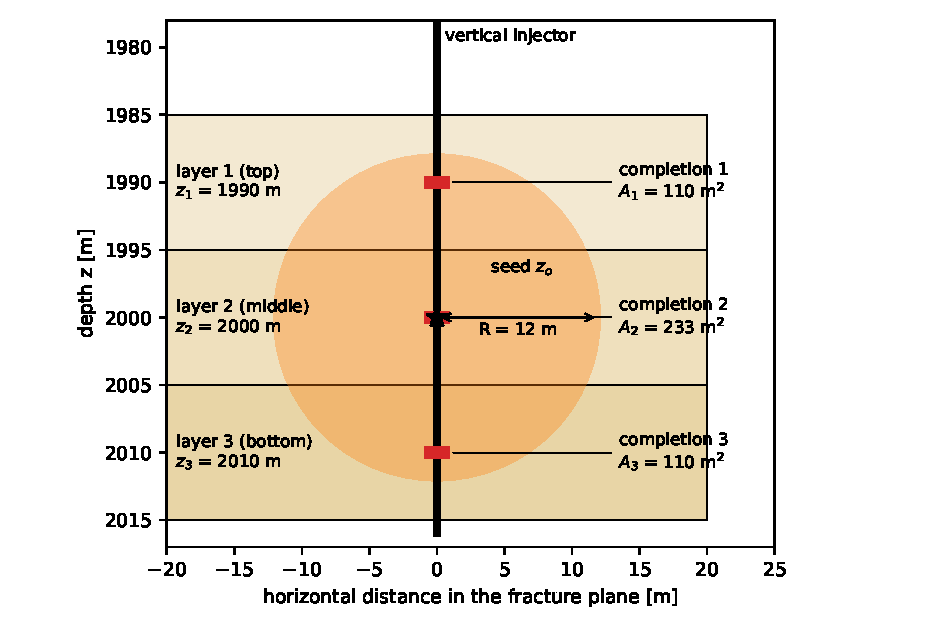
\includegraphics[width=0.72\textwidth]{figs/geometry.pdf}
  \caption{Side view in the fracture plane.  Three layers, one completion per layer, a
  circular fracture of radius \Rfrac~m centred on the middle completion.  $A_k$ is the
  fracture area inside layer~$k$.}
  \label{fig:geometry}
\end{figure}

\begin{table}[ht]
\centering\small
\begin{tabular}{llr}
\toprule
quantity & symbol & value \\
\midrule
permeability (isotropic) & $k$ & \permmD~mD \\
water viscosity, mobility & $\mu$, $\lambda=1/\mu$ & \muCp~cP, \num{2000}~(Pa\,s)$^{-1}$\\
water density (reservoir and fracture model) & $\rho_r$ & \rhor~kg/m$^3$ \\
leak-off distance (legacy: $0.25\Delta x$) & $d$ & \dleak~m \\
leaking fracture faces (legacy) & $n_s$ & 2 \\
Young's modulus, Poisson's ratio & $E$, $\nu$ & \Emod~GPa, \nupois \\
net pressure at the seed & $p_{net}$ & \pnet~bar \\
wellbore radius, Peaceman radius & $r_w$, $r_o=0.198\,\Delta x$ & 0.1~m, \ro~m \\
well $\to$ fracture conductance (ring feed) & $W$ & $\WoverL\sum_k L_k$ \\
injection rate (reservoir volumes) & $Q$ & \Qbase~\rated \\
\bottomrule
\end{tabular}
\caption{Parameters of the example.  All rates are reservoir volumes per day, all potentials
are in bar, and all conductances (including the mobility) are in \cond.}
\label{tab:params}
\end{table}

\subsection{Potentials}

Everything below is written in terms of the potential
\begin{equation}
  \Phi = p - p_o - \rho_r g\,(z-z_o)\qquad[\text{bar}],
  \label{eq:potential}
\end{equation}
where $p_o$ is the reservoir pressure at the seed depth.  This is exactly the quantity the
fracture code uses: \texttt{fracture\_dgh\_}$=g\rho z$ is subtracted from the fracture pressure,
and $g\rho z_r$ from the reservoir pressure (\texttt{Fracture::leakOfRate()}).  The reservoir is
hydrostatic, so the three layer potentials are equal, and we set them to zero:
$\Phi_1=\Phi_2=\Phi_3=0$.  The well potential $\Phiw$ is the potential of the injection pressure
at the seed, $\Phiw = p_{inj}-p_o$, which is what the code calls
\texttt{inj\_press}~$-$~\texttt{dh\_perf}.

\paragraph{Why the overpressures are small.}
An open fracture needs $p_f>\sigma_h$.  This does \emph{not} mean that the fracture is far above
the pressure of the cells it cuts.  With continued injection, the cells around the fracture are
pressurised (and the total stress rises with them through poroelastic back-stress), while the
fracture-to-cell connection has a very large conductance (a large face area over a short
distance, $d=\Delta x/4$).  The quantity that matters for the connections is the fracture-to-cell
potential difference.  At a rate $Q$ it is of order $Q/\sum_k L_k$, which for the numbers here is
a few hundredths of a bar.  We prescribe the open state through the net pressure \pnet~bar that
enters the width (Section~\ref{sec:fracture}) and do not model how it was reached.

%======================================================================
\section{The fracture model}
\label{sec:fracture}
%======================================================================

\subsection{Leak-off conductances}

The area of the disk between depths $a$ and $b$ (relative to the centre) is
\begin{equation}
  A(a,b)=\Big[\,z\sqrt{R^2-z^2}+R^2\arcsin(z/R)\,\Big]_{z=\max(a,-R)}^{z=\min(b,R)} ,
\end{equation}
which gives $A_1=A_3=\Atop$~m$^2$ and $A_2=\Amid$~m$^2$ (total $\pi R^2=\Atot$~m$^2$).
The leak-off model of the code (\texttt{Fracture::updateLeakoff()}, legacy) is
\begin{equation}
  \ell_i = n_s\,\frac{\lambda k\,\Delta A_i}{d}
  \qquad\Longrightarrow\qquad
  L_k=\sum_{i\in k}\ell_i = n_s\,\frac{\lambda k A_k}{d},
  \label{eq:leakcond}
\end{equation}
for every fracture cell $i$ with area $\Delta A_i$, and per layer $k$.  This gives
\[
  L_1=L_3=\Ltop,\qquad L_2=\Lmid,\qquad \textstyle\sum_k L_k=\Ltot\quad\text{\cond}.
\]
For comparison, the matrix CTF of each completion (Peaceman, with mobility) is
\begin{equation}
  M_k=\frac{2\pi k h\,\lambda}{\ln(r_o/r_w)}=\Mk\ \text{\cond}.
\end{equation}
The fracture adds 2.6 to 5.5 times the matrix connectivity to each completion.

\subsection{Width, fracture flow and leak-off}

The width is that of a penny-shaped crack under uniform net pressure (Sneddon),
\begin{equation}
  w(r)=\frac{8(1-\nu^2)}{\pi E}\,p_{net}\sqrt{R^2-r^2},\qquad w_{\max}=\wmax\ \text{mm}.
\end{equation}
The fracture plane is discretised by $96\times96$ square cells (side $0.25$~m), of which those
inside the disk are active.  For each active cell $i$ with potential $\Phi_i$ (here
$\Phi_i=p_i-p_o-\rho_r g(z_i-z_o)$, the fracture's own gravity term), the steady mass balance
is
\begin{equation}
  \sum_{j\in\mathcal N(i)} T_{ij}\,(\Phi_i-\Phi_j)
  + \ell_i\,(\Phi_i-\Phi_{k(i)})
  = w_i\,(\Phiw-\Phi_i),
  \qquad
  T_{ij}=\frac{\lambda}{12/w_i^3+12/w_j^3},
  \label{eq:fracflow}
\end{equation}
with the cubic-law face transmissibility $T_{ij}$.  Here $k(i)$ is the layer holding the cell
centre, and $w_i$ (non-zero only on the ring of cells at $r<0.6$~m) is the well feed, with
$\sum_i w_i=W$.  This is \texttt{Fracture::assemblePressure()} and \texttt{addSource()} with
\texttt{perf\_pressure} control, written in potentials.  The leak-off into layer~$k$ is
\begin{equation}
  q_k=\sum_{i\in k}\ell_i\,(\Phi_i-\Phi_k)=L_k\,(\bar\Phi_{F,k}-\Phi_k),
  \label{eq:qk}
\end{equation}
where $\bar\Phi_{F,k}$ is the leak-off-weighted mean fracture potential over the part of the
fracture in layer~$k$.  Because \eqref{eq:fracflow} is linear, $q_k$ is a linear function of
$\Phiw$ and of the layer potentials $\Phi_k$.  We compute this response once and use it
throughout.

\begin{figure}[ht]
  \centering
  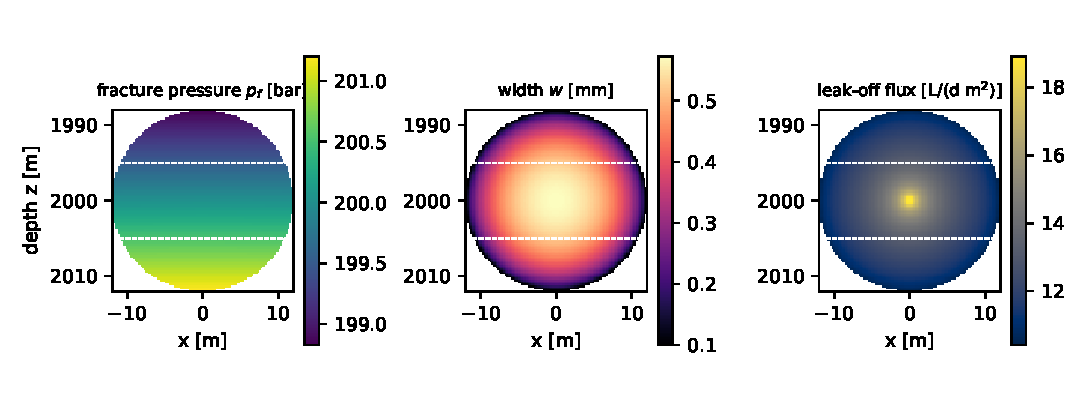
\includegraphics[width=\textwidth]{figs/fracture_fields.pdf}
  \caption{Fracture model at $Q=\Qbase$~\rated: pressure (hydrostatic gradient, top-down),
  width (symmetric), leak-off flux per unit area (dashed lines: layer boundaries).
  The leak-off is positive everywhere, and its mild radial variation comes from the viscous
  pressure drop away from the feed ring.}
  \label{fig:fields}
\end{figure}

\subsection{Reference state at $Q=\Qbase$~\rated}

The fracture is fed from the well, and the matrix completions inject directly.  The well
potential that delivers the rate $Q$ is found from
\begin{equation}
  \sum_k q_k(\Phiw) + \sum_k M_k\,(\Phiw-\Phi_k) = Q .
  \label{eq:refrate}
\end{equation}
The result is $\Phiw=\phiwref$~bar, with a mean fracture potential $\bar\Phi_F=\phiFref$~bar.
The difference of \dpdrop~bar is the pressure drop in the feed ring and in the fracture.  The
leak-off and matrix rates are
\[
  q = (\qftop,\ \qfmid,\ \qfbot),\qquad
  M(\Phiw-\Phi) = (\qmtop,\ \qmmid,\ \qmbot)\quad\text{\rated}.
\]
\textbf{All three layers receive water from the fracture.}  This is what the fracture model
predicts, and it is also what a fully coupled model (fracture cells as unknowns of the flow
problem) would compute.  It is the reference in the following.

%======================================================================
\section{From leak-off to connection factors (the code)}
%======================================================================

\texttt{Fracture::wellIndices\_()} collects the leak-off per reservoir cell and divides it by
the well-to-cell potential difference.  This is the default, \texttt{wi\_upscaling = legacy},
which is assumed up to Section~\ref{sec:conductivity}:

\begin{lstlisting}
double dh_res  = z_cells[i] * gravity_ * dens_cells[i];   // rho_r g z_k
double dh_perf = gravity_ * perf_density * origo_[2];      // rho_r g z_o
double dp_well = (inj_press - dh_perf) - (p_cells[i] - dh_res);
WI  = q_cells[i] / dp_well;           // q_cells: leak-off summed per cell
ctf = WI / mob_cells[i];              // negative WI -> 0
\end{lstlisting}
In potentials this reads
\begin{equation}
  T_k^{\text{leg}}=\lambda\,\mathrm{CTF}_k=\frac{q_k}{\Phiw-\Phi_k}
  =L_k\,\frac{\bar\Phi_{F,k}-\Phi_k}{\Phiw-\Phi_k},
  \qquad T_k^{\text{leg}}\leftarrow 0\ \text{if negative.}
  \label{eq:legacy}
\end{equation}
At the reference state
\[
  T^{\text{leg}}=(\Ttop,\ \Tmid,\ \Tbot)\ \text{\cond},\qquad
  T^{\text{leg}}_k/L_k=(\TLtop,\ \TLmid,\ \TLbot).
\]
These CTFs are passed to Flow (\texttt{addFracturePerforations}) and \emph{added} to the matrix
CTF of the existing completion in \texttt{WellInterface::getTw()}.

%======================================================================
\section{What Flow does with these factors}
%======================================================================

\subsection{Flow's connection model}

For a standard well, Flow computes the flux of connection $k$ as
\begin{equation}
  q^F_k=\big(T_k+M_k\big)\,\big(p_{bhp}+\Delta p^{wb}_k-p_{cell,k}\big),
\end{equation}
where $\Delta p^{wb}_k$ is Flow's hydrostatic wellbore term (computed in
\texttt{StandardWellConnections}) and $p_{cell,k}$ is the cell pressure used by the well model
(oil pressure if oil is active, else gas, else water; see \texttt{getPerfCellPressure}).  Written
with the potential \eqref{eq:potential} and referred to the seed,
\begin{equation}
  \boxed{\;q^F_k=\big(T_k+M_k\big)\,\big(\Phiw^F+s_k-\Phi_k\big)\;}
  \label{eq:flowconn}
\end{equation}
where $s_k$ collects \emph{everything by which Flow's connection potential differs from the
potential $\Phiw$ that the CTF formula \eqref{eq:legacy} assumed}:
\begin{equation}
  s_k = \underbrace{\big(p_{bhp}+\Delta p^{wb}_k\big)-\big(p_{bhp}+\Delta p^{wb}_o\big)
        -\rho_r g(z_k-z_o)}_{\text{wellbore column vs.\ }\rho_r}
        \;-\;\underbrace{\big(p_{cell,k}-p_{w,k}\big)}_{\text{cell pressure vs.\ water pressure}}
        \;+\;\dots
  \label{eq:sk}
\end{equation}
Under rate control, Flow chooses $\Phiw^F$ so that $\sum_k q^F_k=Q$:
\begin{equation}
  \Phiw^F=\frac{Q-\sum_k (T_k+M_k)(s_k-\Phi_k)}{\sum_k (T_k+M_k)} .
  \label{eq:flowphiw}
\end{equation}

\subsection{No mismatch: Flow reproduces the fracture model}

With $s_k=0$ and $\Phi_k=0$, \eqref{eq:flowphiw} gives $\Phiw^F=Q/\sum_k(T_k+M_k)$.  By
construction of \eqref{eq:legacy}, $\sum_k T_k\Phiw=\sum_k q_k$, so $\Phiw^F=\Phiw$, and every
connection carries exactly the reference rate:
\[
  q^F=(\qAtop,\ \qAmid,\ \qAbot)\ \text{\rated}\qquad(\Phiw^F=\phiwA~\text{bar}).
\]
The legacy factors are therefore exact at the state they were computed for, provided Flow
assigns each connection the same potential as the fracture code does.

\subsection{A depth-dependent mismatch: crossflow}

Take a mismatch that is linear in depth,
\begin{equation}
  s_k=-\gamma\,(z_k-z_o),\qquad \gamma=\gammabase~\text{bar/m}\ (=\gammabaseh~\text{bar per 100 m}),
\end{equation}
that is, $s=(+\sTopv,\ 0,\ \sBotv)$~bar.  This is less than $5\,\%$ of the hydrostatic gradient,
and corresponds for instance to a wellbore column that is about 40~kg/m$^3$ lighter than
$\rho_r$ (Section~\ref{sec:sources}).  Because $s$ is antisymmetric and $T_1=T_3$,
$\sum_k(T_k+M_k)s_k=0$ and $\Phiw^F=\phiwC$~bar is unchanged, but the connection rates become
\begin{center}
\begin{tabular}{lrrrr}
\toprule
completion & $\Phiw^F+s_k$ [bar] & fracture part & matrix part & total [\rated] \\
\midrule
1 (top)    & $0.0678$ & \qCftop & \qCmtop & \textbf{\qCtop} \\
2 (middle) & $0.0278$ & \qCfmid & \qCmmid & \qCmid \\
3 (bottom) & $-0.0122$ & \qCfbot & \qCmbot & \textbf{\qCbot} \\
\bottomrule
\end{tabular}
\end{center}
\textbf{The bottom completion produces and the top completion takes the surplus}, although the
fracture model (Figure~\ref{fig:fields}) injects into all layers.
Figure~\ref{fig:profiles} shows why.  The per-connection overpressure is only
$\Phiw^F=Q/\sum_k(T_k+M_k)=\Qbase/\Ttot=\phiwC$~bar.  The mismatch at the bottom completion,
$\gamma(z_3-z_o)=0.04$~bar, is larger than that overpressure, so the bottom connection potential
in Flow falls below the reservoir potential.

\begin{figure}[ht]
  \centering
  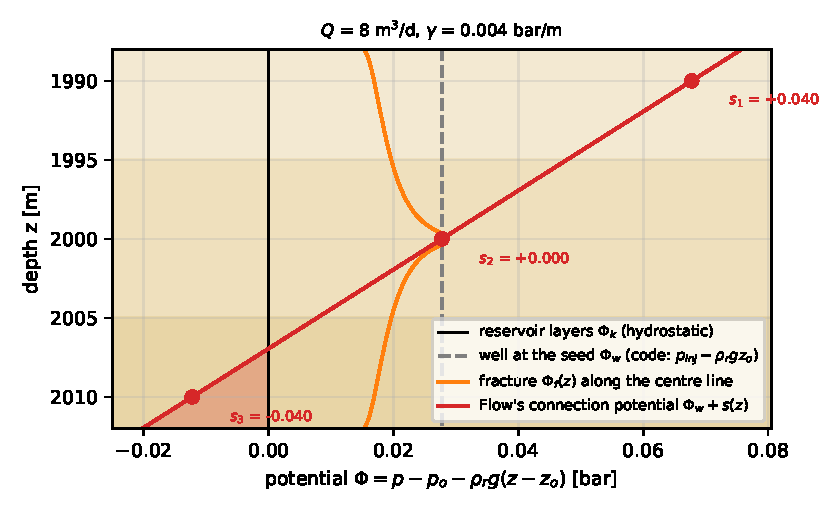
\includegraphics[width=0.78\textwidth]{figs/profiles.pdf}
  \caption{Potentials along the fracture height.  The fracture potential (orange) is above
  the reservoir potential (black) everywhere, so leak-off is positive in all layers.  Flow
  instead assigns each connection the potential $\Phiw+s(z)$ (red).  Below the depth where the
  red line crosses zero, the connection potential is lower than the reservoir potential, and
  Flow produces through the fracture CTF (shaded).}
  \label{fig:profiles}
\end{figure}

\subsection{Critical rate}

From \eqref{eq:flowconn} and \eqref{eq:flowphiw} with $\Phi_k=0$, connection $j$ reverses when
$\Phiw^F+s_j<0$.  The first connection to reverse is the one with the smallest $s_j$, and it
reverses below the critical rate
\begin{equation}
  \boxed{\;Q_{crit}=\sum_k \big(T_k+M_k\big)\,\big(s_k-s_{\min}\big)\;}
  \label{eq:qcrit}
\end{equation}
and for a linear mismatch $s_k=-\gamma(z_k-z_o)$,
$Q_{crit}=\gamma\sum_k (T_k+M_k)\,(z_{\max}-z_k)$.
For the example, $Q_{crit}=\Qcrit$~\rated\ (Figure~\ref{fig:ratesQ}).  Three properties of
\eqref{eq:qcrit} explain the observations:
\begin{enumerate}
\item $Q_{crit}$ is proportional to the \emph{connection factors}.  The fracture factors
  represent leak-off over the whole fracture face, so they are large, and they grow with the
  fracture area.  A larger fracture crossflows up to a larger rate.
\item $Q_{crit}$ is proportional to the mismatch $\gamma$ and to the height spanned by the
  completions (Figure~\ref{fig:qcrit}).
\item The reversal starts at the deepest connection when Flow's connection potential rises more
  slowly with depth than the reservoir potential ($\gamma>0$).  In that case the pattern is
  always injection at the top and production at the bottom.
\end{enumerate}

\begin{figure}[ht]
  \centering
  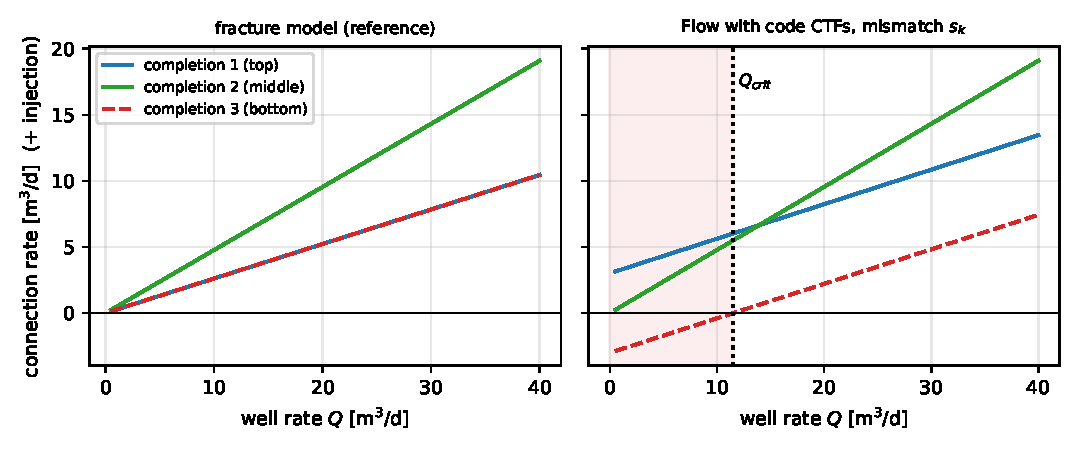
\includegraphics[width=\textwidth]{figs/rates_vs_Q.pdf}
  \caption{Connection rates as a function of the well rate.  Left: fracture model
  (reference), top and bottom coincide.  Right: Flow with the code's CTFs (fixed point of the
  sequential coupling, legacy) and the mismatch $\gamma=\gammabase$~bar/m.  Below
  $Q_{crit}\approx\codeQcrit$~\rated\ the bottom completion produces.}
  \label{fig:ratesQ}
\end{figure}

\begin{figure}[ht]
  \centering
  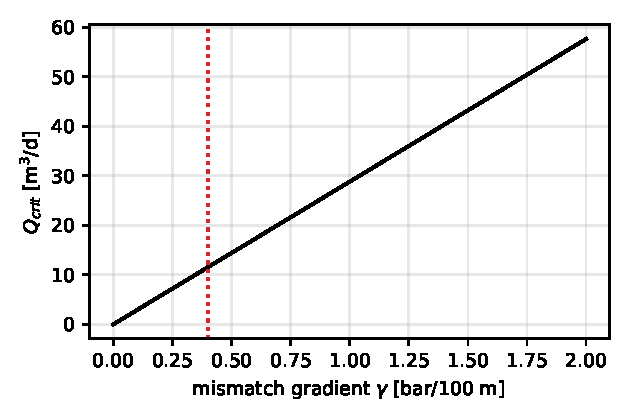
\includegraphics[width=0.5\textwidth]{figs/qcrit.pdf}
  \caption{Critical rate \eqref{eq:qcrit} as a function of the mismatch gradient.}
  \label{fig:qcrit}
\end{figure}

\subsection{Equivalent circuits}

The source of the problem is the change of network topology (Figure~\ref{fig:circuit}).  In
the fracture model, the fracture is a node with its own potential $\PhiF$.  It is fed by the
well and leaks off to the layers, and its potential is set by its own mass balance and its own
fluid column.  In Flow, this node is eliminated.  Each layer is connected straight to the
wellbore through $T_k$, and the potential at the end of that connection is whatever Flow's
wellbore column gives at that depth.  The values $T_k$ make both networks carry the same rates
at one state, but only if the potentials at the connections agree.  The fracture's own column
($\rho_r$, no capillary pressure) is replaced by the wellbore column, so any depth-dependent
difference between the two drives flow through the large fracture factors.

\begin{figure}[ht]
\centering
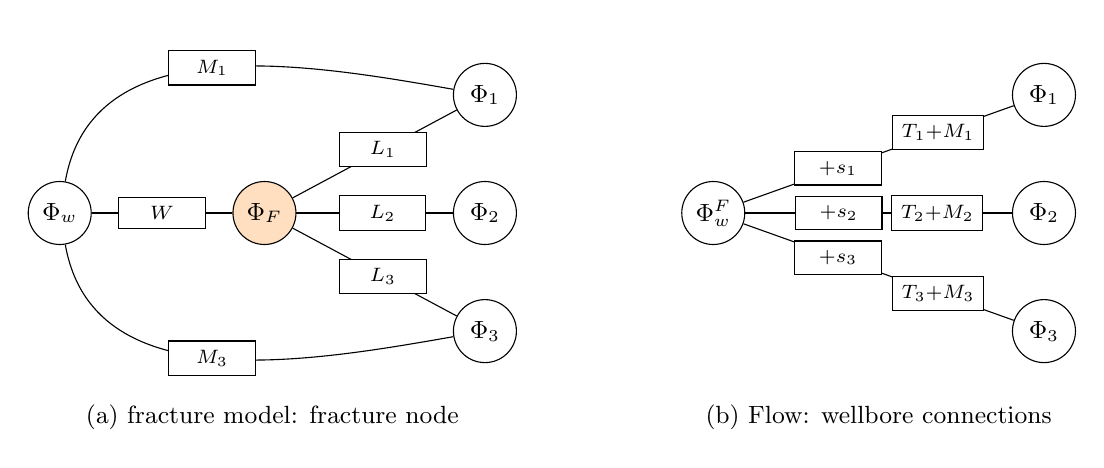
\begin{tikzpicture}[node distance=1.2cm,>=Stealth,
  pot/.style={circle,draw,minimum size=8mm,inner sep=0pt,font=\small},
  res/.style={draw,minimum width=1.1cm,minimum height=4mm,font=\scriptsize,fill=white}]
% left: reference
\node[pot] (w) at (0,0) {$\Phiw$};
\node[pot,fill=orange!25] (f) at (2.6,0) {$\PhiF$};
\node[pot] (l1) at (5.4,1.5) {$\Phi_1$};
\node[pot] (l2) at (5.4,0) {$\Phi_2$};
\node[pot] (l3) at (5.4,-1.5) {$\Phi_3$};
\draw (w) -- node[res] {$W$} (f);
\draw (f) -- node[res,pos=0.55] {$L_1$} (l1);
\draw (f) -- node[res,pos=0.55] {$L_2$} (l2);
\draw (f) -- node[res,pos=0.55] {$L_3$} (l3);
\draw (w) to[out=80,in=170] node[res,pos=0.5] {$M_1$} (l1);
\draw (w) to[out=-80,in=-170] node[res,pos=0.5] {$M_3$} (l3);
\node[font=\small] at (2.7,-2.6) {(a) fracture model: fracture node};
% right: Flow
\begin{scope}[xshift=8.3cm]
\node[pot] (W) at (0,0) {$\Phiw^F$};
\node[pot] (L1) at (4.2,1.5) {$\Phi_1$};
\node[pot] (L2) at (4.2,0) {$\Phi_2$};
\node[pot] (L3) at (4.2,-1.5) {$\Phi_3$};
\draw (W) -- node[res,pos=0.35] {$+s_1$} node[res,pos=0.72] {$T_1{+}M_1$} (L1);
\draw (W) -- node[res,pos=0.35] {$+s_2$} node[res,pos=0.72] {$T_2{+}M_2$} (L2);
\draw (W) -- node[res,pos=0.35] {$+s_3$} node[res,pos=0.72] {$T_3{+}M_3$} (L3);
\node[font=\small] at (2.1,-2.6) {(b) Flow: wellbore connections};
\end{scope}
\end{tikzpicture}
\caption{(a) The fracture model: the fracture is a node with its own potential $\PhiF$ and its
own fluid column.  (b) Flow: the fracture node is removed, and each layer sees the wellbore
potential plus Flow's column term $s_k$ through the large factor $T_k$.  ($M_2$ is omitted
from (a) for clarity.)}
\label{fig:circuit}
\end{figure}

%======================================================================
\section{Where can $s_k$ come from?}
\label{sec:sources}
%======================================================================

Table~\ref{tab:sources} lists the terms by which Flow's connection potential can differ from
the potential the fracture code used.  The example value $\gamma=\gammabase$~bar/m stands for
any of them.

\begin{table}[ht]
\centering\small
\begin{tabular}{p{4.6cm}p{4.3cm}p{5.6cm}}
\toprule
source & $s_k$ & status / magnitude \\
\midrule
Fracture connection created at the seed depth (\texttt{perf.depth = origo\_[2]}), standard
well & $-\rho_r g(z_k-z_o)$, i.e.\ $\gamma\approx0.1$~bar/m &
Fixed in commit \texttt{c9d4b6e} (depth = cell depth).  Only for connections the fracture
\emph{creates}; deck completions keep their depth.  In this example
$Q_{crit}=\Qcritseed$~\rated, and at $Q=\Qbase$ the rates are
$(\qseedtop,\ \qseedmid,\ \qseedbot)$~\rated. \\[2pt]
Wellbore column density $\rho_{wb}$ (Flow) $\neq$ $\rho_r$ (\texttt{dens\_cells}, CTF) &
$(\rho_{wb}-\rho_r)\,g\,(z_k-z_o)$ &
For water injection, Flow uses $\rho_{w,s}/B_w$ at the cell temperature and salinity, so it is
nearly equal to $\rho_r$.  Large as soon as another phase enters the wellbore (gas or CO$_2$
injection, or crossflowing oil or gas), which is a positive feedback.  $\gamma=\gammabase$ for
$\Delta\rho\approx41$~kg/m$^3$. \\[2pt]
Cell pressure in the well model (oil or gas) vs.\ water pressure in the fracture code &
$-(P_{c,k}-P_{c,o})$ &
Zero below the contacts; depth-dependent in transition zones.  Option~2 removes it. \\[2pt]
Lag and damping of the CTFs (\texttt{wellIndicesAvrg}: (new$+2\cdot$old)/3), reservoir change
during the step &
$\Phi_k$ seen by the CTF $\neq$ $\Phi_k$ in Flow &
Not depth-linear by itself, but it is amplified by the singular formula
\eqref{eq:legacy} (Section~\ref{sec:singular}). \\[2pt]
Real, non-hydrostatic layer potentials &
(not a mismatch) &
Physical crossflow through the fracture; the fracture model shows it too
(Section~\ref{sec:singular}). \\
\bottomrule
\end{tabular}
\caption{Contributions to the mismatch $s_k$ in \eqref{eq:flowconn}.}
\label{tab:sources}
\end{table}

In this particular example, all three completions exist in the deck with their own depths, so
the seed-depth term does not apply.  The fracture CTF is added to the existing connection,
which keeps its deck depth.  For a horizontal well, or a vertical well completed only at the
seed, the fracture \emph{creates} the upper and lower connections.  Before the depth fix, those
connections were placed at $z_o$, which gives $\gamma\approx\rho_r g$, about 25 times the
example value, and a crossflow of tens of \rated\ at $Q=\Qbase$~\rated.

%======================================================================
\section{Non-hydrostatic layers and the singular legacy formula}
\label{sec:singular}
%======================================================================

Suppose the layer potentials genuinely differ, e.g.\
$\Phi=(-\deltab,\ 0,\ +\deltab)$~bar (deeper layer at a higher potential).  Then the fracture
\emph{itself} connects the layers.  When $\Phiw$ is low, the bottom layer feeds the fracture
($q_3<0$).  This is physical crossflow, and the fracture model computes it.
The legacy formula \eqref{eq:legacy} divides by $\Phiw-\Phi_3$, which changes sign at a
different well potential ($\Phiw=\Phi_3=\deltab$~bar) than $q_3$ does ($\Phiw=\pwqbzero$~bar;
the two differ by the pressure drop between well and fracture).  Figure~\ref{fig:singular}
shows the consequences:
\begin{itemize}
\item Between the two zeros, $q_3<0$ but $\Phiw-\Phi_3>0$.  The factor is negative and is set
  to zero, so Flow loses the physical inflow from the bottom layer.
\item Just below $\Phiw=\Phi_3$, both are negative, and $T_3=q_3/(\Phiw-\Phi_3)\to+\infty$.  A
  CTF many times $L_3$ is handed to Flow.  Flow then reproduces $q_3$ only if its own
  $\Phiw^F+s_3-\Phi_3$ equals the value used in the formula.  Any lag, damping or mismatch is
  multiplied by this factor, and Flow's rate control pins $\Phiw^F$ near $\Phi_3$, with large
  injection at the top and production at the bottom.
\end{itemize}
This is the regime of low rates ($\Phiw$ close to the layer potentials) in an almost
hydrostatic reservoir.

\begin{figure}[ht]
  \centering
  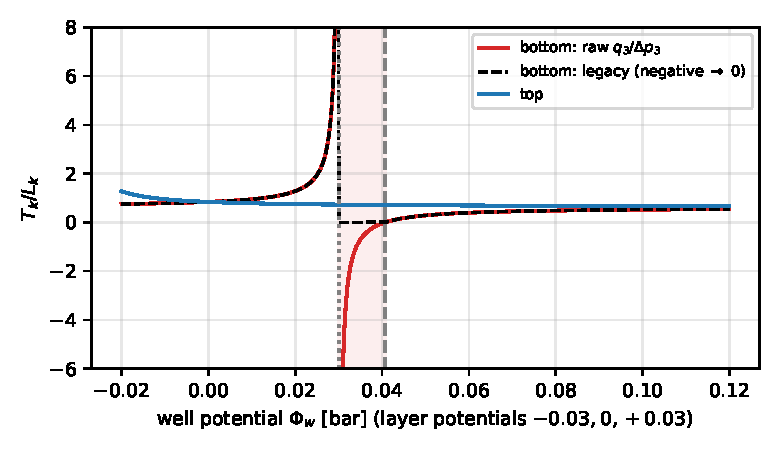
\includegraphics[width=0.62\textwidth]{figs/legacy_singularity.pdf}
  \caption{Legacy factor $T_k/L_k$ as a function of the well potential, with layer
  potentials $(-\deltab,0,+\deltab)$~bar.  Dotted: $\Phiw=\Phi_3$ (pole); dashed: $q_3=0$.
  Shaded: negative factor, set to zero.}
  \label{fig:singular}
\end{figure}

%======================================================================
\section{The sequential coupling in time}
%======================================================================

To see that the reversed connection persists, the layers are given storage.  Each layer is a
tank with storage $C=\Cstore$~m$^3$/bar and support $A_q=\Aqsup$~\cond\ from the rest of the
layer (an almost hydrostatic, well supported reservoir):
\begin{equation}
  C\,\frac{\Phi_k^{n+1}-\Phi_k^n}{\Delta t}=-A_q\,\Phi_k^{n+1}+q^F_k{}^{,n+1},\qquad\Delta t=1~\text{d}.
\end{equation}
Each step reproduces the code's sequence: a fracture solve at Flow's current seed potential and
layer potentials; CTFs from \eqref{eq:legacy}, damped as in \texttt{wellIndicesAvrg}; and an
implicit Flow step with these frozen CTFs under rate control, with $s_k$ as above.  The
reference solves the fracture node implicitly with the layers and has no $s_k$.
Figure~\ref{fig:dynamics} shows the result.  With the legacy factors, the bottom completion
produces throughout ($\dynLbot$~\rated\ at the end, against $+\dynTbot$~\rated\ in the
reference), and the top completion takes \dynLtop~\rated.

\begin{figure}[ht]
  \centering
  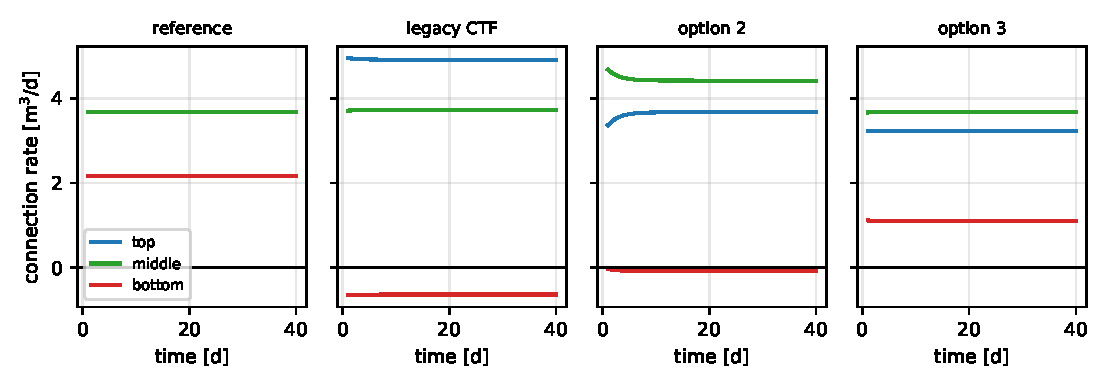
\includegraphics[width=\textwidth]{figs/dynamics.pdf}
  \caption{Connection rates over 40 days of sequential coupling at $Q=\Qbase$~\rated,
  $\gamma=\gammabase$~bar/m.}
  \label{fig:dynamics}
\end{figure}

%======================================================================
\section{Remedies evaluated on the example}
%======================================================================

\paragraph{Option 2 (\texttt{wi\_flow\_column}).}  The CTF is back-calculated against Flow's own
connection potential:
\begin{equation}
  T_k=\frac{q_k}{\Phiw^F+s_k-\Phi_k}.
\end{equation}
At the bottom completion $q_3>0$ but $\Phiw^F+s_3<0$, so the factor is negative and is set to
zero.  The fracture stops feeding the bottom layer in Flow, which is not what the fracture
model says, and the bottom completion now only crossflows through its matrix CTF
($\remTwobot$~\rated).  The rates are $(\remTwotop,\ \remTwomid,\ \remTwobot)$~\rated.
Option~2 removes the \emph{amplification} by the fracture factor, but it inherits the
singularity of Section~\ref{sec:singular}, because it still divides by a potential difference
that can vanish at low rates.

\paragraph{Option 3 (\texttt{wi\_fracture\_pressure}).}  The fracture part of each connection
is driven by the fracture's own potential, shifted with the well:
\begin{equation}
  q^F_k=L_k\big(\Phiw^F+(\bar\Phi_{F,k}-\Phiw)-\Phi_k\big)+M_k\big(\Phiw^F+s_k-\Phi_k\big).
\end{equation}
The mismatch $s_k$ no longer enters the fracture part.  The fracture injects into every layer,
as in the fracture model ($+\remThrfbot$~\rated\ into the bottom layer), and only the ordinary
matrix completion feels Flow's column ($\remThrmbot$~\rated).  That matrix crossflow is Flow's
normal well behaviour and would occur without a fracture.  The rates are
$(\remThrtop,\ \remThrmid,\ \remThrbot)$~\rated, and in time the bottom completion stays at
$+\dynFbot$~\rated\ (Figure~\ref{fig:dynamics}).

\begin{figure}[ht]
  \centering
  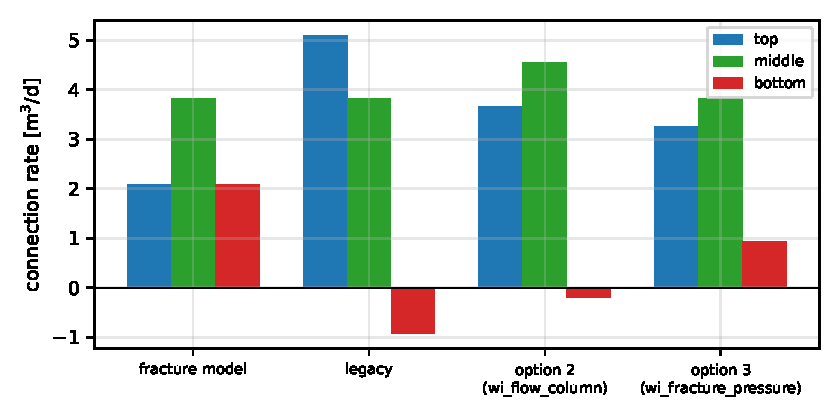
\includegraphics[width=0.72\textwidth]{figs/remedies.pdf}
  \caption{Connection rates at $Q=\Qbase$~\rated\ and $\gamma=\gammabase$~bar/m (fixed point of
  the sequential coupling, frozen layer potentials).}
  \label{fig:remedies}
\end{figure}

%======================================================================
\section{The conductivity mode (\texttt{wi\_upscaling = conductivity})}
\label{sec:conductivity}
%======================================================================

\subsection{What the code does}

In \texttt{conductivity} mode, \texttt{Fracture::wellIndices\_()} does not divide by a potential
difference.  The CTF is the summed leak-off conductance itself, optionally followed by a sign
gate and by one global normalisation factor:
\begin{lstlisting}
ctf = trans_cells[i];                 // sum of leakof_/mobility
const bool not_fed = (q < 0) || (dp_well <= 0 && q > 0);
if (wi_sign_gate && not_fed) ctf = 0; // default: wi_sign_gate = false
sum_q      += q_cells[i];
sum_ctf_dp += ctf * mob * std::max(dp_well, wi_dp_floor);  // floor: 1e4 Pa
...
alpha = std::min(sum_q / sum_ctf_dp, wi_alpha_max);  // if wi_flux_normalization (default on)
perf.ctf *= alpha;                                   // and both sums are positive
\end{lstlisting}
In potentials, with $p_{fl}=\pfloor$~bar (\texttt{wi\_pressure\_floor}) and $\alpha_{\max}=2$,
\begin{equation}
  T_k=\alpha\,L_k\quad(0\ \text{if gated}),\qquad
  \alpha=\min\!\left(\frac{\sum_k q_k}{\sum_k L_k\,\max(\Phiw-\Phi_k,\ p_{fl})},\ \alpha_{\max}\right).
  \label{eq:cond}
\end{equation}
Here $\Phiw-\Phi_k$ is the code's \texttt{dp\_well}: the fracture-side potential difference, or
Flow's own difference when \texttt{wi\_flow\_column} is set.  The factor is positive by
construction, so the singularity of Section~\ref{sec:singular} cannot occur.  The
crossflow mechanism of \eqref{eq:flowconn} is unchanged, however: Flow still applies $T_k$ with
its own connection potential $\Phiw^F+s_k$, and \eqref{eq:qcrit} still holds with $T_k=\alpha L_k$.
What changes is the size of $T_k$, and therefore $Q_{crit}$.

\subsection{Three regimes}

\paragraph{Without normalisation} (\texttt{wi\_flux\_normalization = false}).  Then $T_k=L_k$.
This is larger than the legacy factor ($T^{\text{leg}}_k/L_k\approx0.62$--$0.68$ here), because
$L_k$ ignores the pressure drop between the well and the fracture.  Two consequences follow.
Even without a mismatch, Flow injects \shareCN\ times the modelled leak-off through the
fracture, at a lower well potential ($\Phiw^F=\phiwCN$ instead of \phiwref~bar).  And the
critical rate grows to
\[
  Q_{crit}=\sum_k(L_k+M_k)(s_k-s_{\min})=\QcritNonormAn~\text{\rated}\quad(\text{legacy: }\Qcrit).
\]
At $Q=\Qbase$~\rated, the bottom completion produces \qCNbot~\rated.

\paragraph{Normalisation without floor} ($p_{fl}\to0$).  Here
$\alpha=\sum_k q_k/\big(\sum_k L_k\Phiw\big)=\sum_k T^{\text{leg}}_k/\sum_k L_k=\alphaCF$.
This is the legacy factor averaged over the connections and applied uniformly, so the result is
practically the legacy one ($Q_{crit}\approx\QcritCF$~\rated, bottom \qCFbot~\rated).

\paragraph{Defaults (normalisation with $p_{fl}=\pfloor$~bar).}  At low rates
$\Phiw<p_{fl}$, and the floor takes over the denominator.  With $\sum_k q_k=g\,\Phiw$, where
$g=\gsum$~\cond\ is the fracture model's injectivity,
\begin{equation}
  \alpha=\frac{g}{\sum_k L_k}\,\frac{\Phiw}{p_{fl}},\qquad
  \frac{\text{fracture injection in Flow}}{\text{modelled leak-off}}
  =\frac{\alpha\sum_k L_k\,\Phiw}{g\,\Phiw}=\frac{\Phiw}{p_{fl}}.
  \label{eq:share}
\end{equation}
The normalisation was meant to preserve the total exchange rate.  Below the floor it instead
\emph{throttles} the fracture connections in proportion to $\Phiw/p_{fl}$.  Flow then needs a
higher well potential to place the rate.  The coupled fixed point satisfies
\begin{equation}
  Q=\frac{g}{p_{fl}}\,\Phiw^2+\sum_k M_k\,\Phiw
  \qquad\Longrightarrow\qquad \Phiw=\phiwCD~\text{bar at }Q=\Qbase~\text{\rated},\quad \alpha=\alphaCD,
\end{equation}
so Flow injects only \shareCD\ of the modelled leak-off through the fracture.  Crossflow starts
when $\Phiw$ falls to $-s_{\min}$, which gives
\begin{equation}
  Q_{crit}=\frac{g}{p_{fl}}\,s_{\min}^2+\Big(\sum_k M_k\Big)\,|s_{\min}|=\QcritFloorAn~\text{\rated}.
\end{equation}
This is \emph{quadratic} in the mismatch.  The floor therefore helps against small mismatches
($|s_{\min}|<p_{fl}$), and at $Q=\Qbase$ all completions inject
(\qCDtop, \qCDmid, \qCDbot~\rated).  It gives no protection against large ones: for the
seed-depth mismatch, $\Phiw$ exceeds $p_{fl}$, $\alpha$ returns to $g/\sum_k L_k$, and $Q_{crit}$
is the same $\approx\Qcritseed$~\rated\ as in legacy mode.  Note that the crossflow is suppressed
by misrepresenting the fracture: the BHP in Flow is higher, and the fracture carries less,
than the fracture model says.

\paragraph{Sign gate.}  With the fracture-side \texttt{dp\_well}, the gate never acts in the
mismatch case: the fracture model sees positive leak-off and a positive potential difference
in every layer.  Combined with \texttt{wi\_flow\_column}, the gate removes the fracture part of
every connection where Flow's own potential difference is not positive.  The fracture part then
cannot crossflow.  The remaining production below $Q\approx\QcritCG$~\rated\ in
Figure~\ref{fig:condQ} is the matrix completion alone.

\begin{figure}[ht]
  \centering
  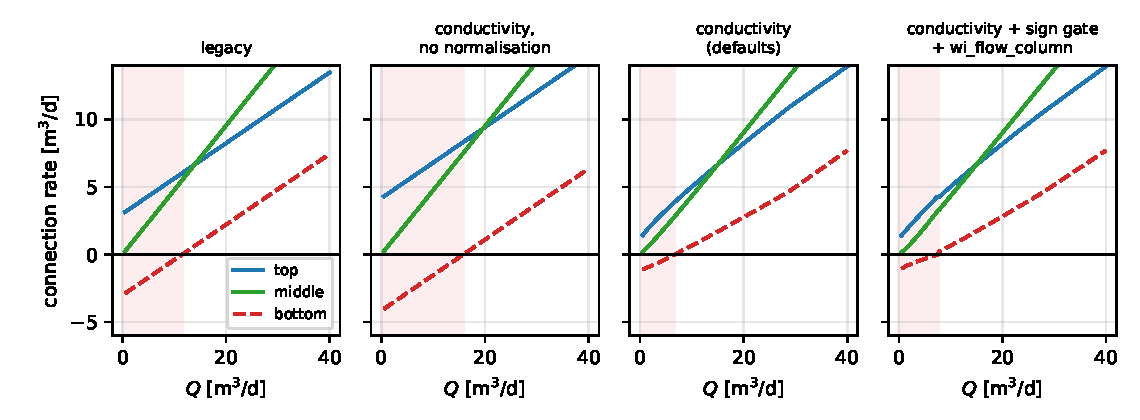
\includegraphics[width=\textwidth]{figs/cond_rates_vs_Q.pdf}
  \caption{Connection rates versus well rate for $\gamma=\gammabase$~bar/m (fixed point of
  the sequential coupling).  Shaded: bottom completion produces.}
  \label{fig:condQ}
\end{figure}

\begin{figure}[ht]
  \centering
  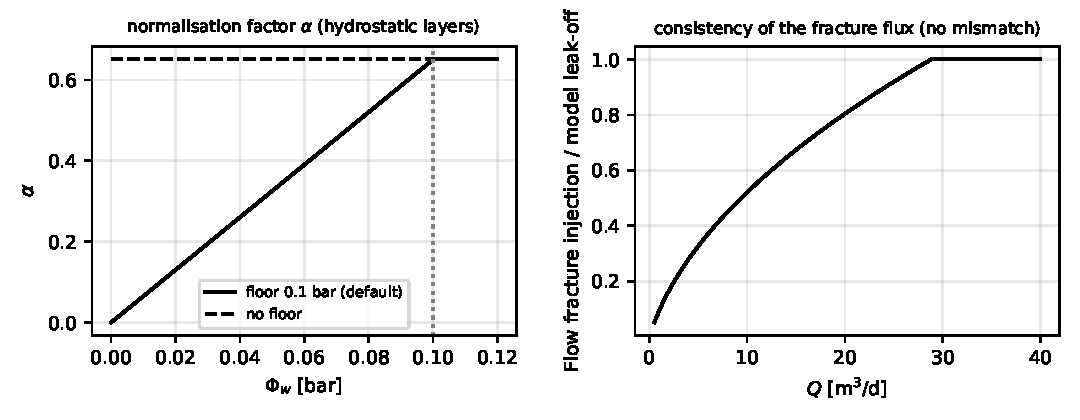
\includegraphics[width=\textwidth]{figs/cond_alpha.pdf}
  \caption{Left: normalisation factor $\alpha$ versus well potential, hydrostatic layers.
  Below the floor (dotted), $\alpha$ falls linearly to zero.  Right: fracture injection in
  Flow relative to the modelled leak-off at the coupled fixed point, without mismatch.  It is
  $\Phiw/p_{fl}$ at low rates, see \eqref{eq:share}.}
  \label{fig:condalpha}
\end{figure}

\subsection{Comparison at $Q=\Qbase$~\rated}

\begin{table}[ht]
\centering\small
\begin{tabular}{lrrrrrr}
\toprule
mode & $\alpha$ & $\Phiw^F$ [bar] & top & middle & bottom & $Q_{crit}$ \\
 & & & \multicolumn{3}{c}{[\rated]} & [\rated] \\
\midrule
fracture model (reference) & -- & \phiwref & \qAtop & \qAmid & \qAbot & -- \\
legacy & -- & \phiwC & \qCtop & \qCmid & \qCbot & \Qcrit \\
conductivity, no normalisation & \alphaCN & \phiwCN & \qCNtop & \qCNmid & \qCNbot & \QcritCN \\
conductivity, no floor & \alphaCF & \phiwCF & \qCFtop & \qCFmid & \qCFbot & \QcritCF \\
conductivity, defaults & \alphaCD & \phiwCD & \qCDtop & \qCDmid & \qCDbot & \QcritCD \\
conductivity + gate + \texttt{wi\_flow\_column} & \alphaCG & \phiwCG & \qCGtop & \qCGmid & \qCGbot & \QcritCG \\
\bottomrule
\end{tabular}
\caption{Fixed points of the sequential coupling with mismatch $\gamma=\gammabase$~bar/m.
$Q_{crit}$ is read from the rate sweeps.}
\label{tab:cond}
\end{table}

\subsection{Non-hydrostatic layers and dynamics}

With genuinely different layer potentials (Section~\ref{sec:singular}), the conductivity factor
has no pole (Figure~\ref{fig:condsing}).  All connections share the same $\alpha$, so the bottom
factor equals the top one.  Two artefacts remain.  First, $\alpha$ jumps to 1 when
$\sum_k q_k\le0$, because the normalisation is skipped.  Second, the sign gate removes the
physical inflow from the bottom layer while $q_3<0$.

In the time-dependent coupling (Figure~\ref{fig:conddyn}), the bottom completion ends at
$\dynCNbot$~\rated\ without normalisation and at $+\dynCDbot$~\rated\ with the defaults
(reference $+\dynTbot$, legacy $\dynLbot$).

\begin{figure}[ht]
  \centering
  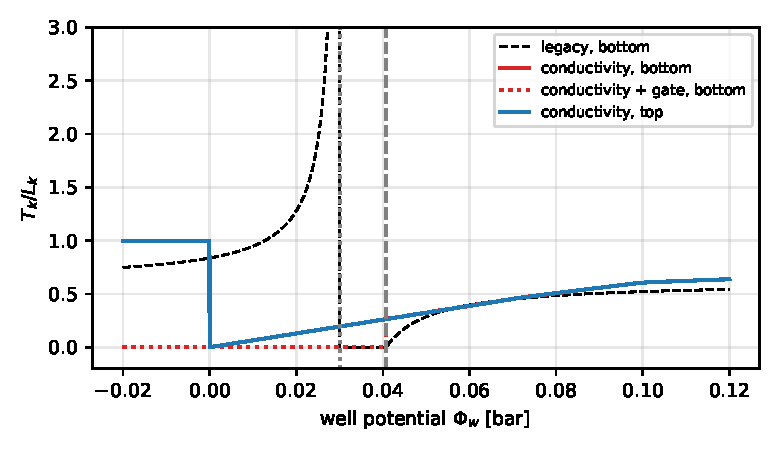
\includegraphics[width=0.62\textwidth]{figs/cond_singularity.pdf}
  \caption{Conductivity factors $T_k/L_k=\alpha$ with layer potentials $(-\deltab,0,+\deltab)$~bar,
  compared with the legacy bottom factor.}
  \label{fig:condsing}
\end{figure}

\begin{figure}[ht]
  \centering
  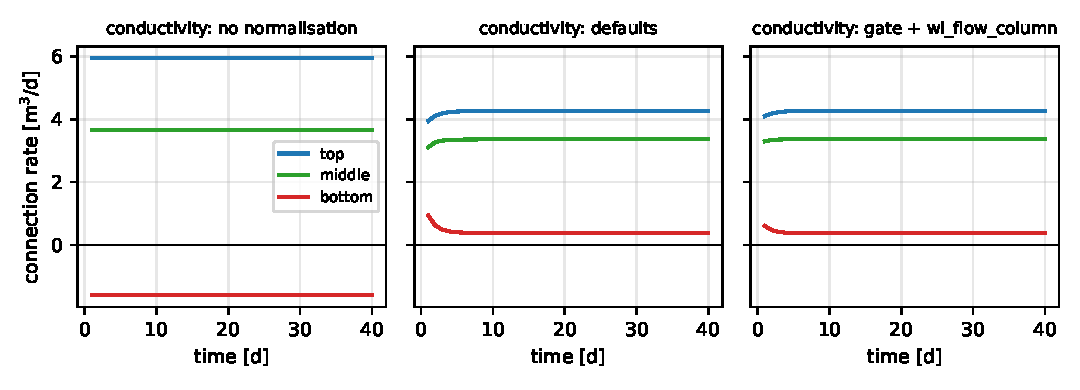
\includegraphics[width=\textwidth]{figs/cond_dynamics.pdf}
  \caption{Sequential coupling over 40 days, conductivity mode, $Q=\Qbase$~\rated,
  $\gamma=\gammabase$~bar/m.}
  \label{fig:conddyn}
\end{figure}

%======================================================================
\section{Formation damage and the m51w deck}
\label{sec:m51w}
%======================================================================

\subsection{Properties from \texttt{test/m51w/TEST.DATA}}

The geometry is now taken from the deck (Figure~\ref{fig:m51wgeom}).  The cells are
$2\times2\times2$~m.  The injector \texttt{B-3H} is completed in K=36--40 (centres
1971--1979~m), and the seed is at K=38 ($z_o=1975$~m).  A circular fracture of radius
$R=\WR$~m again covers three completions (K=37--39); K=36 and K=40 are matrix-only.  The
fracture settings are those of \texttt{params/seq\_implicit\_fb\_robust\_v2\_test3.json}.

\begin{table}[ht]
\centering\footnotesize
\begin{tabular}{p{5.6cm}p{3.6cm}p{5.2cm}}
\toprule
quantity & value & source \\
\midrule
permeability (completed layers), $k_v/k_h$ & 1000~mD, 0.1 & \texttt{EQUALS PERMX}, \texttt{MULTIPLY PERMZ} \\
water density, viscosity, $B_w$ (195~bar) & \Wrhow~kg/m$^3$, \Wmu~cP, \WBw & \texttt{DENSITY}, \texttt{PVTW}, \texttt{EQUIL} \\
mobility (water zone, WOC above the model) & $\lambda=1/\mu_w$ & \texttt{EQUIL} WOC 1000~m \\
rate & \WQs~sm$^3$/d $=\WQ$~\rated & \texttt{WCONINJE} \\
wellbore radius, Peaceman radius, $\ln(r_o/r_w)$ & \Wrw, \Wro~m, \WD & \texttt{COMPDAT} diameter 0.216 \\
matrix CTF per completion & $M_k=\WM$~\cond & Peaceman, $h=2$~m \\
leak-off distance, faces & $d=\Wdleak$~m, $n_s=2$ & \texttt{calculate\_dist}, legacy model \\
leak-off conductance per m$^2$ of fracture & \Wlpa~\cond & $n_s\lambda k/d$ \\
$E$, $\nu$ & 14~GPa, 0.35 & \texttt{YMODULE}, \texttt{PRATIO} \\
net pressure (example choice), $w_{\max}$ & \Wpnet~bar, \Wwmax~mm & Sneddon \\
feed & cells within 1~m of the well & \texttt{well\_source\_all\_perfs}, radius 1.0 \\
filter cake & $k_c=\Wkc$~mD, $\phi_c=\Wphic$, LINRAD & \texttt{WINJDAM} \\
particle concentration & \Wconc~ppm & \texttt{WINJFCNC} \\
\bottomrule
\end{tabular}
\caption{Parameters taken from the m51w deck and its fracture settings.}
\label{tab:m51w}
\end{table}

\begin{figure}[ht]
  \centering
  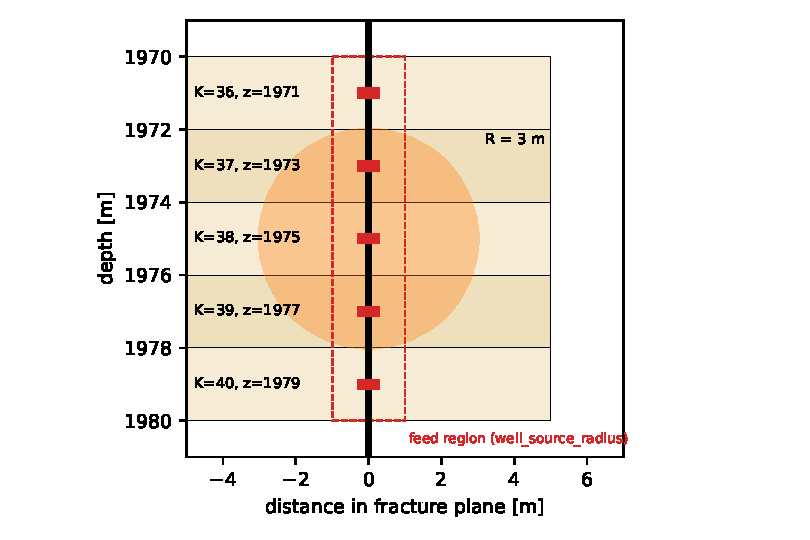
\includegraphics[width=0.55\textwidth]{figs/m51w_geometry.pdf}
  \caption{m51w geometry: five completions in 2~m cells, a fracture of radius \WR~m around the
  seed (K=38), and the feed region of \texttt{well\_source\_all\_perfs}.}
  \label{fig:m51wgeom}
\end{figure}

\paragraph{Why the fracture is open at a small overpressure.}  At the seed, the total
horizontal stress from \texttt{STREQUIL} is $\sigma_h\approx\Wsig$~bar, against a pore pressure
of \Wpres~bar.  Water is injected at 30~$^\circ$C into a 90~$^\circ$C reservoir
(\texttt{WTEMP}, \texttt{RTEMPVD}).  The thermal stress reduction of fully cooled rock,
$E\alpha_T\Delta T/(1-\nu)\approx\Wdsig$~bar, exceeds the effective stress.  The cooled region
therefore fractures at a pressure close to the reservoir pressure, which is the situation
assumed throughout this note.

\subsection{The margin in m51w}

The fracture leak-off conductance is $\sum_k L_k=\WLtot$~\cond\ for only $28$~m$^2$ of
fracture: \Wlpa~\cond\ per m$^2$ at 1000~mD and $d=0.5$~m.  At the deck rate, the overpressure
per connection relative to the adjacent cells is $\Phiw=\Wphiw$~bar.  That is about 1/\Wratio\
of the hydrostatic difference across a single 2~m cell (\Whyd~bar).  With frozen layer
potentials, the critical mismatch at the deck rate is only $\gamma=\Wgcl$~bar/m for legacy
(about \Wgclpct\,\% of the hydrostatic gradient) and \Wgcc~bar/m for conductivity
(Figure~\ref{fig:m51wqcrit}).

\begin{figure}[ht]
  \centering
  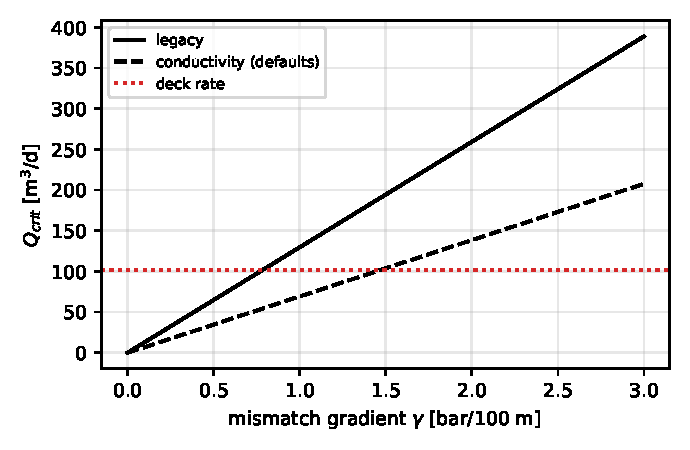
\includegraphics[width=0.55\textwidth]{figs/m51w_qcrit.pdf}
  \caption{m51w, frozen layer potentials: critical rate \eqref{eq:qcrit} against the mismatch
  gradient.  The deck rate is crossed at $\gamma=\Wgcl$ (legacy) and \Wgcc~bar/m (conductivity).}
  \label{fig:m51wqcrit}
\end{figure}

\paragraph{The layers re-equilibrate.}  The frozen-layer picture does not hold over Flow's
time steps.  With $k=1000$~mD, the pressure diffusion time over 10~m is of the order of
seconds.  Each layer's pressure therefore follows its own injection, and a layer that
receives less water stays at a lower pressure, which restores its drive.  We represent each
completed layer by a tank with storage $C=\WC$~m$^3$/bar, drainage $A_q=\WAq$~\cond\ to the far
field, and vertical coupling $T_v=\WTv$~\cond\ to the neighbouring layers.  These are
order-of-magnitude estimates from the deck: drainage to the free bottom boundary, and
$k_v=100$~mD over a $20\times20$~m$^2$ near-well area.  The layers then rise by about 0.2~bar
above their initial potential.  Sustained crossflow needs a mismatch large enough to overcome
this build-up, which gives the quasi-steady critical mismatch
\[
  \gamma_{crit}=\WgssLeg~\text{(legacy)},\quad \WgssCon~\text{(conductivity)},\quad
  \WgssOpt~\text{bar/m (option 3)},
\]
i.e.\ 20--30\,\% of the hydrostatic gradient.  Below that, a mismatch only skews the
distribution.  At $\gamma=0.01$~bar/m, for example, the top completion takes \WskewLegtop~\rated\
and the bottom one \WskewLegbot~\rated\ (legacy), against 10.5 each in the reference.  Mismatches
of 20--30\,\% of the hydrostatic gradient come from the seed-depth placement of connections the
fracture creates (before the depth fix), or from gas in the wellbore column.  They do not come
from the small density or capillary differences of a water-filled deck.  The physical drainage
to the free bottom boundary (\texttt{BCPROP 6 FREE}) gives a potential gradient of
$\approx\Wbeta$~bar/m that \emph{decreases} with depth, which favours injection at the bottom.

With option~3, which is what the m51w settings use (\texttt{wi\_fracture\_pressure = true}),
the completion that reverses first is K=40, the matrix-only completion below the fracture.
The fracture part is immune to $s_k$, but it pressurises the fractured layers, and through the
vertical coupling also K=40, while K=40's matrix connection still sees Flow's column.

\paragraph{Layer pressurisation and the legacy formula.}  For a mismatch above the threshold,
$\gamma=\Wgamma$~bar/m in the dynamics below, the two effects reinforce each other in legacy
mode.  Flow injects more into the top fractured layer (K=37), which raises that layer's
potential above the well potential ($\Phi_{37}=\WLegNphiTop$ vs.\ $\Phiw=\WLegNphiw$~bar).  The
fracture model, which is solved with Flow's layer potentials, then sees \emph{inflow} from K=37
($q=\WLegNqmodTop$~\rated).  The legacy formula divides a negative leak-off by a negative
potential difference and returns a large positive factor, so Flow keeps injecting
\WLegNqfTop~\rated\ there.  K=39 is the opposite case: the model leaks off \WLegNqmodLow~\rated\
there, but Flow injects only \WLegNqfLow~\rated\ (Figure~\ref{fig:m51wflowmodel}, left).  This
is the singular regime of Section~\ref{sec:singular}, reached through the layers' own response.

\subsection{Formation damage (\texttt{WINJDAM})}

Two cakes grow independently in the code.

\paragraph{Matrix completions} (\texttt{WellFilterCake}, LINRAD).  The matrix share of the
injected water of each connection deposits particles on the perforation area
$A_c=2\pi r_wL$:
\begin{equation}
  \Delta h=\frac{q^{mat}_k\,c\,\chi\,\Delta t}{A_c(1-\phi_c)},\qquad
  S_k\mathrel{+}=\frac{K}{k_c}\ln\frac{r_w+h+\Delta h}{r_w+h},\qquad
  M_k\leftarrow M_k\,\frac{D}{D+S_k},
\end{equation}
with $K/k_c=\WKkc$, $D=\ln(r_o/r_w)=\WD$, and the crossflow factor
$\chi=\sum q/\sum q^+$.  The multiplier is applied to the matrix part of $T_w$ only
(\texttt{WellInterface::getTw}).  Because $D$ is small (2~m cells) and $K/k_c=100$, the damage
is fast: at the seed completion the multiplier is \WmTen\ after 10 days and \WmHundred\ after 100
days (Figure~\ref{fig:m51wdamage}).

\paragraph{Fracture faces} (\texttt{Fracture::updateFilterCakeProps}, \texttt{updateLeakoff}).
Each fracture cell accumulates a cake from its \emph{modelled} positive leak-off, scaled by
Flow's fracture rate (\texttt{scale\_filtrate}).  The cake acts in series with the reservoir
path on each face:
\begin{equation}
  \Delta h_{c,i}=\frac{\max(\ell_i(\Phi_i-\Phi_{k(i)}),0)\,f_s\,c\,\Delta t}{\Delta A_i(1-\phi_c)},\qquad
  \ell_i=n_s\Big/\Big(\frac{d}{\lambda k\Delta A_i}+\frac{h_{c,i}/n_s}{\lambda k_c\Delta A_i}\Big).
\end{equation}
The fracture face area is much larger, so this cake grows slowly: the leak-off conductance is
at \WLHundred\ of its clean value after 100 days at the seed layer.

\begin{figure}[ht]
  \centering
  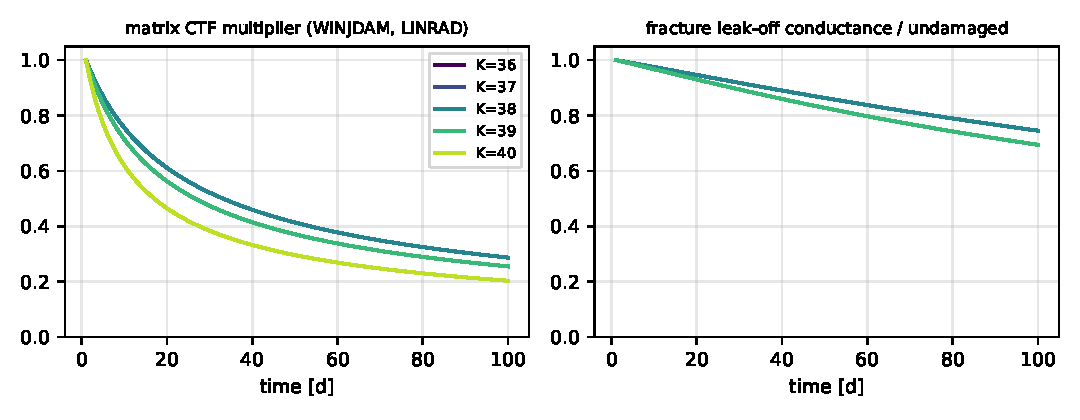
\includegraphics[width=\textwidth]{figs/m51w_damage.pdf}
  \caption{Reference run with \texttt{WINJDAM}: matrix CTF multipliers (left) and fracture
  leak-off conductance relative to the clean fracture (right).}
  \label{fig:m51wdamage}
\end{figure}

\subsection{Effects of the damage on crossflow}

Figure~\ref{fig:m51wdyn} compares 100 days of sequential coupling with and without
\texttt{WINJDAM}, at $\gamma=\Wgamma$~bar/m.

\begin{enumerate}
\item \textbf{The well pressure rises.}  The conductances fall, so the BHP rises to place the
  rate ($\Phiw$: \WRefNphiwlast\ $\to$ \WRefDphiwlast~bar in the reference), and every connection
  gets more margin against the mismatch.  The quasi-steady critical mismatch at the
  day-100 damage state increases to \WgssdLeg\ (legacy), \WgssdCon\ (conductivity) and
  \WgssdOpt~bar/m (option~3).
\item \textbf{Only injecting completions are damaged.}  The cake grows only where water goes in.
  A crossflowing completion stays clean (K=40 keeps a multiplier of \WLegDmBot\ in the legacy
  run), while the injecting ones lose 60--85\,\% of their matrix CTF.  The net effect is still
  less crossflow, because the rising BHP dominates: at K=40 the rate goes from \WLegNbotlast\ to
  \WLegDbotlast~\rated\ (legacy) and from \WOptNbotlast\ to \WOptDbotlast~\rated\ (option~3).
  In conductivity mode it changes sign, from \WConNbotlast\ to $+$\WConDbotlast~\rated.
\item \textbf{Injection moves into the fracture.}  The matrix-only completions K=36 and K=40
  drop from 10.5 to \WRefDbotlast~\rated\ in the reference, and the fracture takes the rest.
\item \textbf{The fracture cake goes where the model leaks off, not where Flow injects.}  In
  the legacy run, the model sees inflow from K=37 ($q=\WLegDqmodTop$~\rated), so no cake forms
  there (leak-off conductance \WLegDLrelTop\ of clean), while Flow injects \WLegDqfTop~\rated\
  through it.  K=39, where the model leaks off, is damaged to \WLegDLrelBot\ of clean.  The
  damage thus pushes even more of Flow's injection to the top: \WLegNqfTop\ $\to$
  \WLegDqfTop~\rated\ (Figure~\ref{fig:m51wflowmodel}, right).  This is a positive feedback on
  the skew, built on the inconsistency between Flow's connection rates and the fracture model's
  leak-off.  With option~3 the two are consistent, and the fracture cake is evenly distributed.
\end{enumerate}

\begin{figure}[ht]
  \centering
  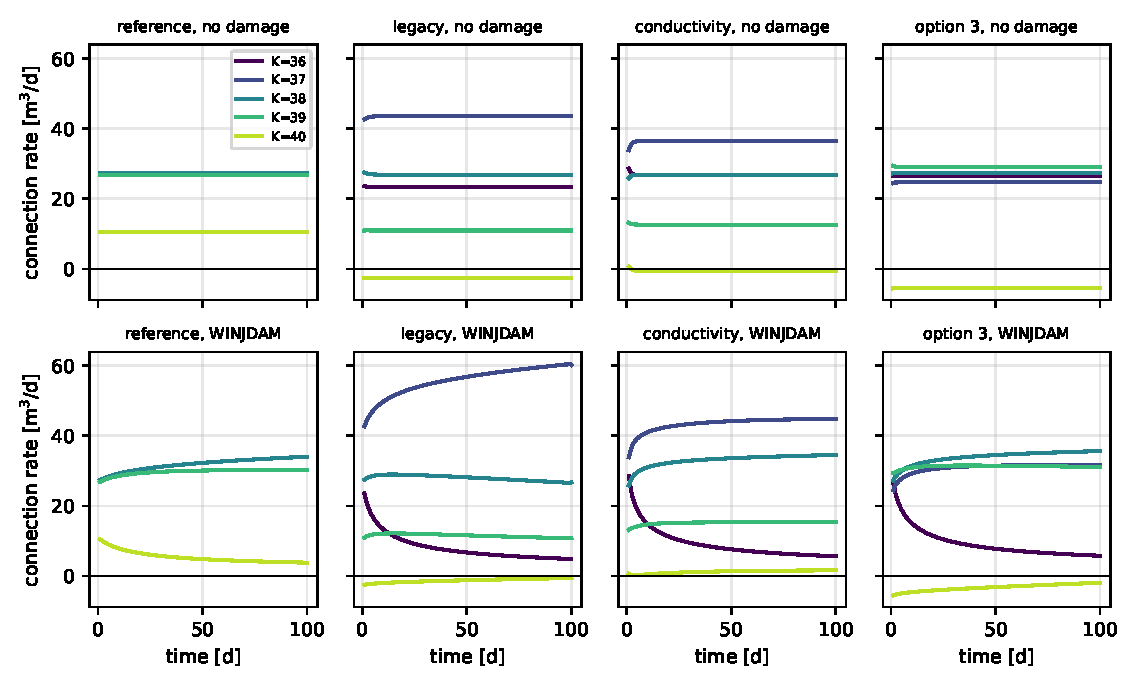
\includegraphics[width=\textwidth]{figs/m51w_dynamics.pdf}
  \caption{m51w properties, sequential coupling over 100 days at the deck rate with
  $\gamma=\Wgamma$~bar/m.  Top: no damage.  Bottom: \texttt{WINJDAM}/\texttt{WINJFCNC} as in the
  deck.  Total connection rates per completion.}
  \label{fig:m51wdyn}
\end{figure}

\begin{figure}[ht]
  \centering
  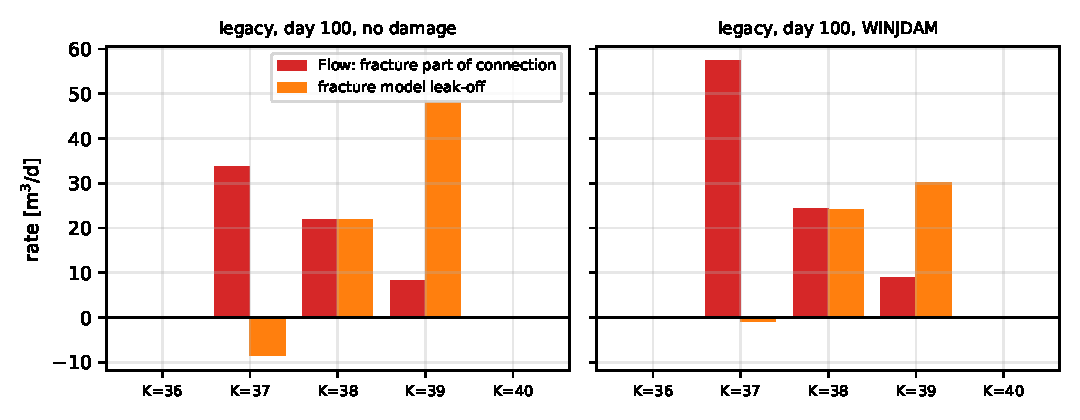
\includegraphics[width=\textwidth]{figs/m51w_flow_vs_model.pdf}
  \caption{Legacy mode, day 100: fracture part of Flow's connection rates against the
  fracture model's own leak-off per completion.  The two disagree in sign at K=37, and the
  cake is laid down according to the model.}
  \label{fig:m51wflowmodel}
\end{figure}

\subsection{What this means for m51w}

\begin{itemize}
\item The overpressure per connection is tiny (0.03~bar), but the layers' own build-up
  protects against small mismatches.  Sustained crossflow needs a mismatch of 20--30\,\% of the
  hydrostatic gradient.  Such mismatches came from the seed-depth placement of new connections
  before the depth fix.  They can also occur when the fracture grows beyond K=36--40, so that
  new connections are created.
\item With the m51w settings (option~3), the fracture connections are immune to the mismatch.
  Remaining crossflow goes through the matrix-only completions outside the fracture, or is
  physical (non-hydrostatic layer potentials).
\item \texttt{WINJDAM} reduces crossflow mainly by raising the BHP.  In legacy and conductivity
  modes it can also reinforce a skew, because the fracture cake follows the fracture model's
  leak-off rather than Flow's connection rates.
\item Model limitations: tanks instead of a grid, a prescribed fracture size and width, and no
  thermal effects on the fluids (none are in the deck).  The numbers indicate orders of
  magnitude and directions, not a prediction of the m51w run.
\end{itemize}

%======================================================================
\section{Summary}
%======================================================================

\begin{enumerate}
\item The legacy CTF $T_k=q_k/(\Phiw-\Phi_k)$ is exact only at the state it was computed for,
  and only if Flow gives every connection the potential $\Phiw$ that the formula assumed.
\item Flow applies the factors with its own wellbore column and cell pressures.  Any
  depth-dependent difference $s_k$ acts as an extra driving potential on the fracture factors.
  Under rate control, the deepest connection reverses for $Q<Q_{crit}=\sum_k(T_k+M_k)(s_k-s_{\min})$.
\item The fracture factors are large (leak-off over the whole face), while the overpressure per
  connection at low rates is $Q/\sum_k(T_k+M_k)$, a few hundredths of a bar.  A mismatch of the
  same order (here $\pm0.04$~bar over $\pm10$~m) is enough to produce injection at the top and
  production at the bottom.
\item Without the depth fix, connections created by the fracture were placed at the seed depth
  ($\gamma\approx\rho_r g$), which gives $Q_{crit}$ of hundreds of \rated\ for this small
  fracture.
\item When the layer potentials truly differ, the fracture model also crossflows (physical).
  The legacy formula is singular there, and it zeroes or inflates the bottom factor.
\item \texttt{wi\_upscaling = conductivity} removes the pole but not the mechanism.  Without
  normalisation, $T_k=L_k$ is larger than the legacy factor, so it crossflows more
  ($Q_{crit}=\QcritCN$ vs.\ \Qcrit~\rated).  With the default normalisation, the pressure floor
  scales the fracture connections by $\Phiw/p_{fl}$ at low rates.  This lowers $Q_{crit}$
  (\QcritCD~\rated) only by making Flow inject less through the fracture than the fracture model
  computes, and it does not help against mismatches larger than the floor.
\item Driving the fracture part with the fracture's own pressure (option~3) removes the
  fracture-induced crossflow.  Option~2 removes the mismatch but keeps the singular division.
  The structural alternative is the embedded coupling, where the fracture node stays in the
  flow problem.
\item With the m51w properties, the layers' own pressure build-up raises the threshold for
  sustained crossflow to a mismatch of 20--30\,\% of the hydrostatic gradient.
  \texttt{WINJDAM} raises it further through a higher BHP.  In legacy and conductivity modes,
  however, the fracture cake is deposited according to the fracture model's leak-off, not
  Flow's connection rates, which can reinforce an existing skew.
\end{enumerate}

\appendix
\section{Reproducing the numbers}
All numbers and figures are generated by \texttt{crossflow\_example.py} and
\texttt{m51w\_case.py} in this directory (run both, then \texttt{pdflatex crossflow\_example.tex}).
The two-dimensional fracture solve uses \texttt{scipy.sparse}; the response to the well and
layer potentials is computed once and then used for every rate, coupling iteration and time
step.

\end{document}
